\chapter{Resultados}


\section{Introdução aos Resultados}

Este capítulo apresenta os resultados obtidos a partir da aplicação dos métodos de classificação de texto analisados neste estudo, incluindo tanto técnicas baseadas em Argmax quanto diversos métodos de aprendizado de máquina. A avaliação do desempenho desses métodos é crucial para compreender sua eficácia na classificação de descrições de produtos em português, utilizando o dataset RETAILPRODUCTDESCRIPTION-PTBR especialmente preparado para este fim.

Inicialmente, será apresentada uma análise detalhada dos resultados obtidos com o método Argmax, explorando diferentes configurações de vetorização, tokenização e normalização, e como estas afetam o desempenho do método em termos de acurácia e F1-Score Macro. Esta análise é complementada por testes estatísticos ANOVA e regressão OLS para quantificar o impacto de cada configuração.

Em seguida, procede-se à análise detalhada de cada método de aprendizado de máquina empregado neste estudo, incluindo SVM, Árvores de Decisão, Naive Bayes, k-Nearest Neighbors e Regressão Logística. Para cada um desses métodos, o capítulo inicia com a descrição do processo de ajuste fino (fine-tuning) dos hiperparâmetros, visando otimizar o desempenho em termos de acurácia e F1-Score Macro. 

Após a fase de ajuste fino, serão apresentados os resultados gerais alcançados, focando no desempenho otimizado de cada método e como as diferentes configurações impactam esse desempenho. A análise inclui uma exploração da relevância estatística dos resultados, utilizando testes ANOVA e regressão OLS para quantificar e comparar o impacto de cada configuração de parâmetros. Esta abordagem metódica permite uma compreensão aprofundada da eficácia de cada método de aprendizado de máquina dentro do contexto específico deste estudo, bem como fornece insights valiosos sobre a importância das escolhas de pré-processamento e configuração na classificação de textos.


Finalmente, o capítulo conclui com uma comparação geral dos resultados de todos os métodos analisados, oferecendo uma visão integrada do desempenho relativo de cada técnica. Esta seção de resultados gerais visa identificar os métodos mais promissores para a classificação de textos curtos em português, considerando as particularidades do dataset em estudo. Discussões sobre as limitações dos resultados, considerações para a interpretação dos dados e sugestões para pesquisas futuras também serão abordadas, fornecendo um panorama completo dos achados e sua implicação para o campo do processamento de linguagem natural e aprendizado de máquina.
.
\subsection{Introdução à Avaliação do Método Argmax}

Para a avaliação do método Argmax, diversas combinações de parâmetros foram examinadas. O foco desta análise reside na determinação de configurações ótimas que influenciam a classificação de textos, especificamente nas descrições de produtos em português. As combinações de parâmetros selecionadas para estudo incluem:

\begin{itemize}
\item \textbf{Método de Vetorização:} Abordagens distintas para a vetorização dos textos foram consideradas, visando a transformação eficaz dos dados textuais em formatos numéricos adequados para processamento algorítmico. As abordagens analisadas são:
\begin{enumerate}
\item Binária
\item Frequência de Termos (TF)
\item Frequência de Termos-Inverso da Frequência nos Documentos (TF-IDF)
\end{enumerate}
\item \textbf{Alcance de N-Gramas:} Dois alcances de n-gramas foram avaliados para investigar a influência da contextualização em diferentes níveis de granularidade:
\begin{enumerate}
\item Unigramas (1,1)
\item Bigramas (1,2)
\end{enumerate}
\item \textbf{Normalização:} A influência da normalização dos vetores de características foi examinada sob duas condições:
\begin{enumerate}
\item Sem normalização
\item Com normalização L2
\end{enumerate}
\end{itemize}
A análise dos resultados apresentados na Tabela \ref{resultadoargmax} revela insights importantes sobre o desempenho dos métodos baseados em Argmax sob diferentes configurações de vetorização, tokenização e normalização. Observa-se uma variação significativa no desempenho, tanto em termos de acurácia quanto de F1 Score, o que indica a sensibilidade desses métodos às escolhas de pré-processamento e representação dos dados.

A configuração que utiliza o método binário com tokenização de bigramas ([1, 2]) e sem normalização (None) alcançou a maior acurácia média (89.56%) e F1 Score médio (70.09%). Isso sugere que a representação binária combinada com a análise de pares de palavras adjacentes é particularmente eficaz para capturar a informação contextual necessária para a classificação de texto no conjunto de dados analisado. A baixa variação no desempenho (CV) para esta configuração reforça sua estabilidade e robustez.

Por outro lado, a aplicação da normalização L2 juntamente com o método binário e tokenização de unigramas ([1, 1]) resultou em um desempenho significativamente inferior, com acurácia média de apenas 19.07% e F1 Score médio de 25.39%. Este resultado destaca a importância da escolha apropriada de normalização, que neste caso, prejudicou substancialmente o desempenho do modelo.

Interessantemente, a abordagem TermFrequency, especialmente quando combinada com normalização L2 e tokenização de bigramas ([1, 2]), também mostrou resultados promissores, com acurácia média de 79.65% e F1 Score médio de 55.56%. Isso indica que, para certas configurações, a consideração da frequência dos termos pode proporcionar um aumento significativo no desempenho da classificação.

Os métodos TFIDF, conhecidos por sua capacidade de ponderar termos baseando-se em sua importância relativa nos documentos, apresentaram um bom desempenho geral, particularmente na configuração com tokenização de bigramas ([1, 2]) e normalização L2, alcançando uma acurácia média de 82.76% e F1 Score médio de 59.83%. Esse resultado reforça a eficácia do TFIDF em destacar termos significativos para a classificação de texto.

Em suma, os resultados indicam uma clara vantagem em explorar representações baseadas em bigramas para capturar a estrutura linguística dos textos. Além disso, a escolha do método de vetorização e a decisão sobre a aplicação de normalização são críticas para o desempenho dos modelos baseados em Argmax, exigindo uma avaliação cuidadosa para maximizar a acurácia e o F1 Score. A análise detalhada dessas configurações fornece insights valiosos para a seleção de técnicas de pré-processamento e representação de texto em tarefas de classificação automatizada.

\begin{table}[H]
\centering
\caption{Resultados Argmax}
\label{resultadoargmax}
\begin{tabular}{lllrrrr}
\toprule
Método & Tokenização & Normalização & \multicolumn{2}{c}{Acurácia (\%)} & \multicolumn{2}{c}{F1 Score (\%)} \\
\cmidrule(lr){4-5} \cmidrule(lr){6-7}
 &  &  & Média & CV & Média & CV \\
\midrule
Binary & [1, 1] & None & 75.31 & 0.44 & 58.77 & 3.15 \\
Binary & [1, 1] & L2 & 19.07 & 2.40 & 25.39 & 2.04 \\
Binary & [1, 2] & None & 89.56 & 0.21 & 70.09 & 1.91 \\
Binary & [1, 2] & L2 & 31.30 & 1.48 & 33.82 & 1.77 \\
TermFrequency & [1, 1] & None & 63.76 & 0.41 & 23.44 & 2.05 \\
TermFrequency & [1, 1] & L2 & 77.05 & 0.24 & 52.31 & 2.46 \\
TermFrequency & [1, 2] & None & 66.68 & 0.28 & 27.08 & 1.69 \\
TermFrequency & [1, 2] & L2 & 79.65 & 0.29 & 55.56 & 2.61 \\
TFIDF & [1, 1] & None & 70.64 & 0.28 & 32.10 & 2.25 \\
TFIDF & [1, 1] & L2 & 78.37 & 0.32 & 55.20 & 2.47 \\
TFIDF & [1, 2] & None & 74.57 & 0.33 & 37.67 & 1.53 \\
TFIDF & [1, 2] & L2 & 82.76 & 0.29 & 59.83 & 2.52 \\
\bottomrule
\end{tabular}
\end{table}


\section{Análise dos Resultados do Método Argmax}

Os resultados obtidos pelas diversas combinações de parâmetros para o método Argmax foram analisados com base em duas métricas principais: acurácia e F1 Score Macro. Os gráficos gerados oferecem uma perspectiva visual do desempenho dessas combinações sob diferentes configurações.

\subsection{Análise dos Boxplots}

Os boxplots das acurácias (Figura \ref{fig:boxplot_acuracia}) demonstram uma variância relativamente baixa entre as combinações de parâmetros testadas. Observou-se a presença de poucos outliers, indicando que a maioria das configurações apresenta um desempenho consistente. As combinações que utilizam o método binário sem normalização destacaram-se por apresentar as melhores acurácias, enquanto aquelas com normalização L2 mostraram-se menos eficazes.

Similarmente, os boxplots dos F1 Scores Macro (Figura \ref{fig:boxplot_f1score}) revelam que as configurações com bom desempenho em acurácia tendem também a exibir resultados satisfatórios no F1 Score Macro. Este padrão sugere que as configurações selecionadas são capazes de manter um equilíbrio razoável na performance entre as diversas classes, mesmo considerando o desbalanceamento presente no conjunto de dados.

As diferenças na ordenação das combinações de parâmetros ao considerar acurácia e F1 Score Macro revelam insights sobre o comportamento dos modelos Argmax sob diferentes configurações. Observa-se que as combinações utilizando o método binário sem normalização (binary-[1, 2]-None) apresentam a maior acurácia média (89,56%) e também o maior F1 Score Macro (70,09%), indicando um desempenho superior tanto na classificação geral quanto na capacidade de tratar classes de maneira equitativa.

Por outro lado, combinações que empregam normalização L2 com o método binário (binary-[1, 1]-l2 e binary-[1, 2]-l2) mostram-se menos eficazes, com as menores acurácias médias (19,07% e 31,30%, respectivamente) e F1 Scores Macro (25,39% e 33,82%, respectivamente). Isso sugere que a normalização L2 pode não ser adequada para a vetorização binária no contexto do método Argmax.

Interessantemente, enquanto a vetorização TF e TFIDF sem normalização (termfrequency-[1, 1]-None, termfrequency-[1, 2]-None, tfidf-[1, 1]-None, e tfidf-[1, 2]-None) apresentam um desempenho intermediário em termos de acurácia, elas não seguem a mesma ordem ao considerar o F1 Score Macro. Em particular, a combinação tfidf-[1, 2]-None sobressai com um F1 Score Macro significativamente maior (37,67%) em comparação com sua acurácia (74,57%), indicando uma maior efetividade na classificação equitativa das classes.

Ao analisar as configurações que utilizam normalização L2 com métodos TF e TFIDF (termfrequency-[1, 1]-l2, termfrequency-[1, 2]-l2, tfidf-[1, 1]-l2, e tfidf-[1, 2]-l2), percebe-se um aumento notável tanto na acurácia quanto no F1 Score Macro, culminando na combinação tfidf-[1, 2]-l2 com as maiores pontuações em ambas as métricas (82,76% de acurácia e 59,83% de F1 Score Macro). Isso reforça a ideia de que a normalização L2 pode ser benéfica para a vetorização TF e TFIDF, contrariamente ao observado com o método binário.

Essas diferenças sublinham a importância de uma seleção cuidadosa dos parâmetros na otimização dos modelos Argmax, destacando como a escolha da técnica de vetorização e a decisão de aplicar normalização podem impactar significativamente tanto o desempenho geral quanto a justiça na classificação das classes desbalanceadas.

\subsection{Análise do Gráfico Scatter}

O gráfico scatter, relacionando acurácia e F1 Score Macro (Figura \ref{fig:scatter_acuracia_f1score}), permitiu a identificação de quatro grupos distintos de configurações, divididos conforme a mediana de cada métrica. As configurações que utilizam os métodos TF e TFIDF com normalização localizaram-se no quadrante superior direito, indicando um desempenho superior em ambas as métricas. Por outro lado, as combinações binárias com normalização situaram-se no quadrante inferior esquerdo, apresentando os piores resultados tanto em acurácia quanto em F1 Score Macro.

Conclui-se que a normalização apresenta um impacto significativo no desempenho dos métodos de vetorização TF e TFIDF, enquanto as configurações binárias alcançam melhores resultados sem essa intervenção. Portanto, a escolha de normalizar ou não as representações vetoriais deve ser considerada cuidadosamente, a fim de otimizar o desempenho dos modelos de classificação de texto.

\begin{figure}[H]
    \centering
    \includegraphics[width=0.8\textwidth]{images/ArgmaxAcuráciaTodos.png}
    \caption{Boxplot das acurácias das combinações Argmax.}
    \label{fig:boxplot_acuracia}
\end{figure}

\begin{figure}[H]
    \centering
    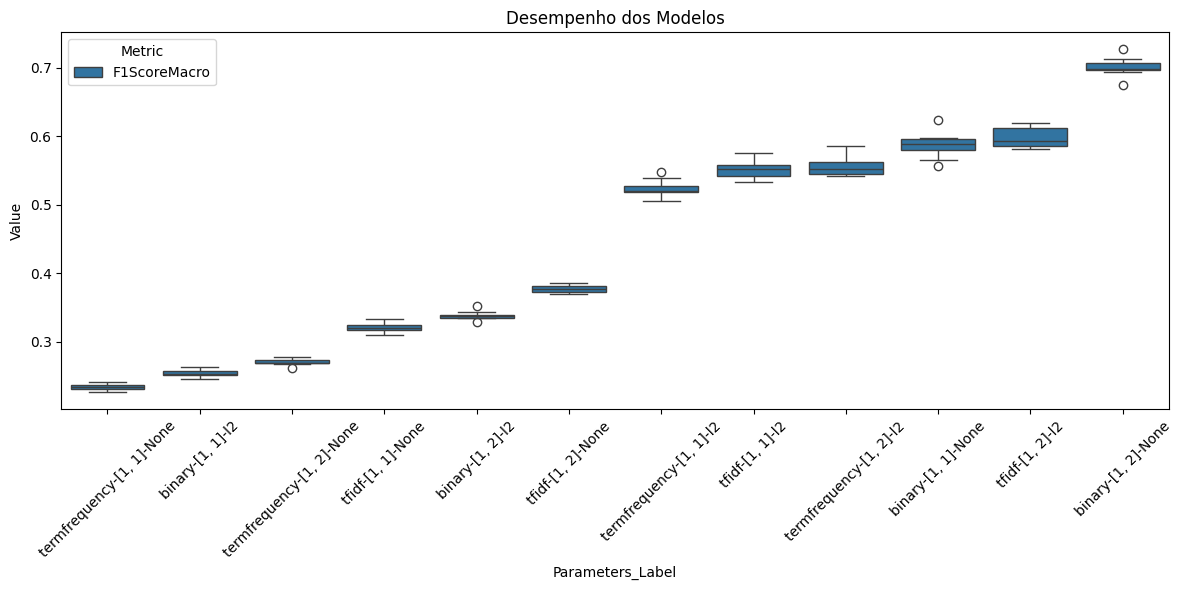
\includegraphics[width=0.8\textwidth]{images/ArgmaxF1ScoreTodos.png}
    \caption{Boxplot dos F1 Scores Macro das combinações Argmax.}
    \label{fig:boxplot_f1score}
\end{figure}

\begin{figure}[H]
    \centering
    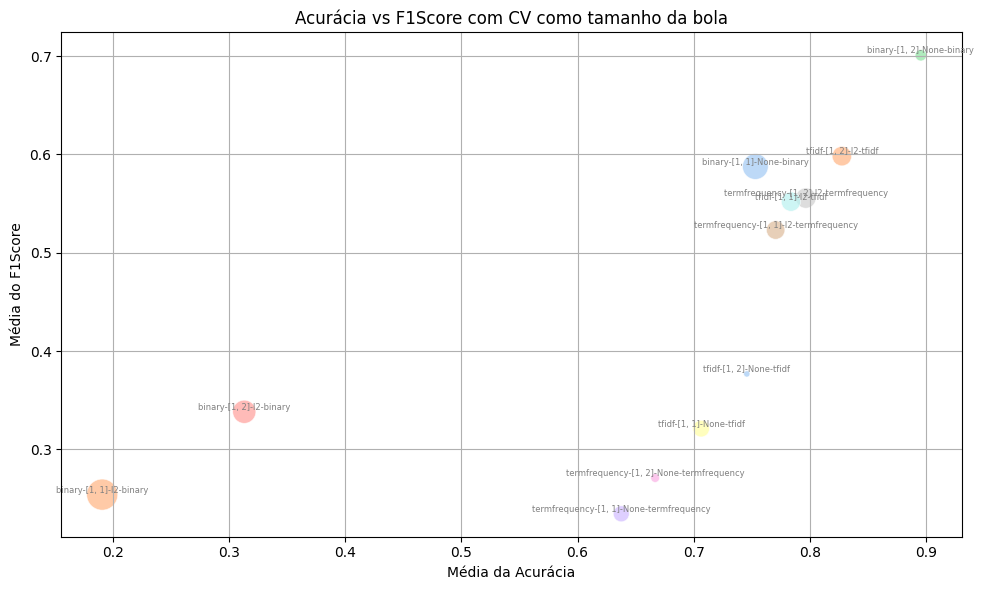
\includegraphics[width=0.8\textwidth]{images/ArgmaxScatterTodos.png}
    \caption{Scatter plot relacionando acurácia e F1 Score Macro das combinações Argmax.}
    \label{fig:scatter_acuracia_f1score}
\end{figure}

\begin{table}[H]
\centering
\caption{Comparação de \# Acurácia e \# F1Score para Configurações do Método Argmax}
\label{tab:resultadocomparativo}
\footnotesize % Diminui a fonte da tabela
\begin{tabular}{llllrrrr}

Método & Tokenização & Normalização &  \# Acurácia &  \# F1Score &  Acurácia (\%) &  F1ScoreMacro (\%) \\

Binary & [1, 2] & None &  1 & 1 & 89.56 & 70.09 \\
TFIDF & [1, 2] & L2 & 2 & 2 & 82.76 & 59.83 \\
TF & [1, 2] & L2 & 3 & 4 & 79.65 & 55.56 \\
TFIDF & [1, 1] & L2 & 4 & 5 & 78.37 & 55.20 \\
TF & [1, 1] & L2 & 5 & 6 & 77.05 & 52.31 \\
Binary & [1, 1] & None & 6 & 3 & 75.31 & 58.77 \\
TFIDF & [1, 2] & None & 7 & 7 & 74.57 & 37.67 \\
TFIDF & [1, 1] & None & 8 & 9 & 70.64 & 32.10 \\
TF & [1, 2] & None & 9 & 10 & 66.68 & 27.08 \\
TF & [1, 1] & None & 10 & 12 & 63.76 & 23.44 \\
Binary & [1, 2] & L2 & 11 & 8 & 31.30 & 33.82 \\
Binary & [1, 1] & L2 & 12 & 11 & 19.07 & 25.39 \\

\end{tabular}
\end{table}

A Tabela \ref{tab:resultadocomparativo} oferece uma análise detalhada do desempenho das configurações do método Argmax, evidenciando as variações nas classificações de acurácia e F1ScoreMacro. Notavelmente, a abordagem `Binary [1, 2] None` se destaca, ocupando a primeira posição em ambas as métricas, o que demonstra sua eficiência em termos de precisão geral e tratamento equitativo das classes. As discrepâncias entre as classificações de acurácia e F1ScoreMacro para algumas configurações reforçam a importância de avaliar os modelos sob diversas métricas para alcançar um balanço entre precisão global e justiça na classificação.



% Análise do Método Argmax
\section{Análise dos Resultados do Método Argmax}
\subsection{Resultado Geral}
Apresentação do desempenho geral do método Argmax, incluindo acurácia e F1-Score Macro, com análise estatística relevante.

\subsection{Impacto do Método de Vetorização}
\subsubsection{Box Plot}
\subsubsection{Tabela de Desempenho}
\subsubsection{Análise ANOVA}

\subsection{Impacto da Tokenização}
\subsubsection{Box Plot}
\subsubsection{Tabela de Desempenho}
\subsubsection{Análise ANOVA}

\subsection{Impacto da Normalização}
\subsubsection{Box Plot}
\subsubsection{Tabela de Desempenho}
\subsubsection{Análise ANOVA}

\subsection{Discussão dos Resultados do Argmax}
Discussão sobre os resultados obtidos com o método Argmax, interligando com a literatura existente e interpretando os achados.

% Repita a estrutura acima para cada método de ML analisado
% Exemplo para um método de ML: SVM
\section{Análise dos Resultados do Método SVM}
\subsection{Resultado Geral}
\subsubsection{Box Plot}
\subsubsection{Tabela de Desempenho}
\subsubsection{Análise ANOVA}

\subsection{Impacto do Método de Vetorização}
\subsubsection{Box Plot}
\subsubsection{Tabela de Desempenho}
\subsubsection{Análise ANOVA}

\subsection{Impacto da Tokenização}
\subsubsection{Box Plot}
\subsubsection{Tabela de Desempenho}
\subsubsection{Análise ANOVA}

\subsection{Impacto da Normalização}
\subsubsection{Box Plot}
\subsubsection{Tabela de Desempenho}
\subsubsection{Análise ANOVA}

\subsection{Discussão dos Resultados do SVM}
Discussão detalhada dos resultados obtidos com o método SVM, fazendo conexões com estudos anteriores e teorias relevantes.

% Adicione seções similares para outros métodos de ML aqui

\section{Resultado Geral Comparativo}
Esta seção compara os resultados obtidos de todos os métodos analisados, destacando as principais diferenças e semelhanças em termos de desempenho.

\subsection{Box Plots Comparativos}
\subsection{Tabelas de Desempenho Comparativas}
\subsection{Análise ANOVA Geral}

\section{Considerações sobre os Resultados}
Discussão sobre as limitações dos resultados, possíveis viéses e sugestões para pesquisas futuras.

\section{Conclusões da Seção de Resultados}
Sumário dos achados mais significativos desta seção, reiterando a contribuição dos resultados para os objetivos da pesquisa.

Principais Achados
Desempenho dos Métodos de Vetorização:

O método tfidf com a configuração de ngram_range de [1, 2] e norm=l2 apresentou o melhor desempenho em termos de acurácia (R² ajustado de 1.000 para interação de nível 3), indicando a eficácia desta abordagem na captura de informações contextuais e na normalização dos dados para a classificação de texto.
Impacto da Normalização:

A normalização (norm=l2) mostrou ter um impacto significativo na melhoria do desempenho dos modelos, especialmente quando combinada com o método tfidf e ngram_range de [1, 2]. Isso sugere que a normalização é crucial para a eficácia da classificação em datasets com variações na escala dos dados.
Efeito do Ngram Range:

A utilização de bigramas ([1, 2]) melhorou o desempenho em comparação com o uso exclusivo de unigramas ([1, 1]), o que é evidenciado pelo aumento da acurácia e do F1-Score Macro. Isso destaca a importância de considerar as relações entre palavras adjacentes para a classificação de textos.
Comparação entre Métodos de Vetorização:

tfidf superou binary e termfrequency em termos de desempenho, especialmente quando aplicado com bigramas e normalização L2. Isso indica que a ponderação da frequência dos termos inversa à frequência dos documentos ajuda a destacar termos mais informativos para a classificação.
Variação no Desempenho:

O desempenho variou significativamente entre as diferentes configurações testadas, como evidenciado pelos coeficientes de variação e pelos intervalos de confiança nos resultados da regressão OLS. A escolha cuidadosa dos parâmetros é, portanto, essencial para otimizar os modelos de classificação de texto.
Conclusões e Recomendações
Os resultados do experimento sublinham a complexidade da modelagem eficaz em tarefas de classificação de texto e a necessidade de uma seleção cuidadosa dos métodos de pré-processamento e vetorização. A análise sugere que:

A combinação de tfidf com bigramas ([1, 2]) e normalização L2 parece ser a abordagem mais promissora para a classificação de texto, oferecendo um equilíbrio ideal entre precisão e capacidade de generalização.
A normalização dos dados desempenha um papel crítico na melhoria do desempenho dos modelos, especialmente em conjuntos de dados com características de alta dimensionalidade e variabilidade.
As interações entre os parâmetros de vetorização e normalização têm um impacto significativo no desempenho, indicando a importância de experimentar combinações desses parâmetros para encontrar a configuração ótima.
Para pesquisas futuras, recomenda-se explorar a aplicação desses insights em conjuntos de dados diversificados e avaliar o impacto de técnicas adicionais de pré-processamento e modelagem, como a lematização e o uso de modelos de linguagem pré-treinados, para melhorar ainda mais a acurácia e a robustez dos sistemas de classificação de texto.



\subsection*{Regressão Logística: Seleção de Hiperparâmetros}

O total de combinações testadas foi 80. Estas foram geradas a partir de todas as combinações viáveis de hiperparâmetros \textit{penalty}, com valores \textcolor{red}{\{"none", "l1", "l2", "elasticnet"\}}, \textit{C} com valores \{0.1,1,10,100,1000\}, \textit{peso da classe} com valores \{None, 'balanced'\} e \textit{razão l1} com valores \{0.1, 0.3, 0.5, 0.7, 0.9\}, apenas quando a \textit{penalty} é elasticnet.

Após a execução dos modelos, os resultados foram agrupados por hiperparâmetro e apresentados nas Tabelas \ref{tab01} a \ref{tab03}. Observou-se que não aplicar penalidade tem a melhor média de acurácia e o menor desvio padrão. Por isso, a avaliação do hiperparâmetro $l1\_ratio$ não é relevante. Similarmente, a não aplicação de pesos tem a melhor média e o menor desvio padrão. Finalmente, o valor 100 para o hiperparâmetro C apresenta a melhor acurácia e o menor desvio padrão.
\textcolor{red}{
Os hiperparâmetros selecionados foram C igual a 100, solver igual a saga, sem penalidade e sem peso de classe.}

% Tabela 1
\begin{table}[!htpp]
	\vspace{0.3cm}
    %\centering
  \caption{Resultados de média e desvio padrão de acurácias do hiperparâmetro Penalty}
	\vspace{-0.6cm}
	\label{tab01}
	\renewcommand{\arraystretch}{1.2}
	\begin{center}
\begin{tabular}{ccc}
\hline
\textbf{valor} &	\textbf{média \%}	& \textbf{desvio \%}\\
\hline		
      none & 87.69 & 2.31 \\
        l2 & 79.15 & 22.12 \\
elasticnet & 76.59 & 22.23 \\
        l1 & 73.16 & 28.56
 \\
\hline
\end{tabular}
\end{center}
%\small\textbf{Fonte:} Os autores.
\end{table}

% Tabela 2
\begin{table}[!htpp]
	\vspace{0.3cm}
    %\centering
  \caption{Resultados de média e desvio padrão de acurácias do hiperparâmetro Peso da Classe}
	\vspace{-0.6cm}
	\label{tab02}
	\renewcommand{\arraystretch}{1.2}
	\begin{center}
\begin{tabular}{ccc}
\hline
\textbf{valor} &	\textbf{média \%}	& \textbf{desvio \%}\\
\hline		
        none & 81.06 & 15.59 \\
    balanced & 74.62 & 26.15 \\
\hline
\end{tabular}
\end{center}
%\small\textbf{Fonte:} Os autores.
\end{table}

% Tabela 3
\begin{table}[!htpp]
	\vspace{0.3cm}
    %\centering
  \caption{Resultados de média e desvio padrão de acurácias do hiperparâmetro C}
	\vspace{-0.6cm}
	\label{tab03}
	\renewcommand{\arraystretch}{1.2}
	\begin{center}
\begin{tabular}{ccc}
\hline
\textbf{valor} &	\textbf{média \%}	& \textbf{desvio \%}\\
\hline		
 100.0 & 88.31 & 0.89 \\
   1.0 & 86.11 & 2.70 \\
1000.0 & 83.62 & 1.02 \\
  10.0 & 83.09 & 18.46 \\
   0.1 & 53.57 & 29.71 \\
\hline
\end{tabular}
\end{center}
%\small\textbf{Fonte:} Os autores.
\end{table}

\subsection*{Máquina de Vetores de Suporte SVM: Seleção de Hiperparâmetros}

Um total de 80 combinações foi avaliado. Estas foram geradas a partir de todas as combinações viáveis de hiperparâmetros \textit{kernel}, com valores \textcolor{red}{\{"linear", "poli", "rbf", "sigmóide"\}}, \textit{C} com valores \{0.1,1,10,100,1000\}, \textit{peso da classe} com valores \{None, 'balanced'\} e \textit{grau} com valores \{2,3,5,8,13\}, apenas para o \textit{kernel} poli.

Após avaliar todas as combinações, foram geradas as Tabelas \ref{tab04} a \ref{tab06}. Observou-se que o kernel com o melhor resultado é o sigmóide, com maior média de acurácia e menor desvio padrão. O melhor hiperparâmetro C é o valor 100. Como o modelo polinomial não foi escolhido, não há necessidade de escolher o hiperparâmetro de grau. Finalmente, o modelo não se distinguiu entre balancear ou não as classes.

\textcolor{red}{
Os hiperparâmetros selecionados foram C igual a 100, kernel igual a sigmóide e peso da classe igual a balanced.}

% Tabela 4
\begin{table}[!htpp]
	\vspace{0.3cm}
    %\centering
  \caption{Resultados de média e desvio padrão de acurácias do hiperparâmetro Kernel}
	\vspace{-0.6cm}
	\label{tab04}
	\renewcommand{\arraystretch}{1.2}
	\begin{center}
\begin{tabular}{ccc}
\hline
\textbf{valor} &	\textbf{média \%}	& \textbf{desvio \%}\\
\hline		
      sigmóide & 87.35 & 1.32 \\
    rbf & 85.32 & 3.20 \\
 linear & 84.87 & 7.98 \\
   poli & 45.18 & 30.78 \\
\hline
\end{tabular}
\end{center}
%\small\textbf{Fonte:} Os autores.
\end{table}

% Tabela 5
\begin{table}[!htpp]
	\vspace{0.3cm}
    %\centering
  \caption{Resultados de média e desvio padrão de acurácias do hiperparâmetro C}
	\vspace{-0.6cm}
	\label{tab05}
	\renewcommand{\arraystretch}{1.2}
	\begin{center}
\begin{tabular}{ccc}
\hline
\textbf{valor} &	\textbf{média \%}	& \textbf{desvio \%}\\
\hline		
 100 & 66.45 & 29.18 \\
1000 & 64.44 & 30.77 \\
  10 & 63.16 & 31.14 \\
   1 & 60.88 & 32.23 \\
   0.1 & 31.30 & 34.65 \\
\hline
\end{tabular}
\end{center}
%\small\textbf{Fonte:} Os autores.
\end{table}

% Tabela 6
\begin{table}[!htpp]
	\vspace{0.3cm}
    %\centering
  \caption{Resultados de média e desvio padrão de acurácias do hiperparâmetro Peso da Classe}
	\vspace{-0.6cm}
	\label{tab06}
	\renewcommand{\arraystretch}{1.2}
	\begin{center}
\begin{tabular}{ccc}
\hline
\textbf{valor} &	\textbf{média \%}	& \textbf{desvio \%}\\
\hline		
    balanced & 56.87 & 35.58 \\
        none & 56.86 & 33.09 \\
\hline
\end{tabular}
\end{center}
%\small\textbf{Fonte:} Os autores.
\end{table}

\chapter{Resultados e Discussões}

\section{Introdução}

Neste capítulo, são apresentados os resultados obtidos a partir da aplicação das metodologias descritas anteriormente, com foco na avaliação do desempenho dos modelos de classificação de texto. Os objetivos principais deste estudo são revisitados para contextualizar os achados, e uma visão geral das seções seguintes é fornecida.

\section{Apresentação dos Resultados}

\subsection{Análise Descritiva dos Dados}

Após o pré-processamento e a limpeza dos dados, realizou-se uma análise descritiva aprofundada para entender melhor as características do conjunto de dados final utilizado nos modelos de classificação.

\subsection{Resultados do Modelo de Classificação}

\subsubsection{Desempenho dos Modelos}

Os resultados do desempenho de cada modelo de classificação são apresentados, utilizando métricas de avaliação como Acurácia e F1-Score Macro. Tabelas e gráficos são empregados para facilitar a comparação entre os modelos.

\subsubsection{Comparação entre Modelos}

Discussão comparativa do desempenho dos modelos, destacando aqueles que apresentaram melhor desempenho e as métricas em que se destacaram.

\subsection{Avaliação da Seleção de Modelos e Hiperparâmetros}

Análise do impacto que diferentes configurações de hiperparâmetros tiveram no desempenho dos modelos e justificativa para a escolha do modelo final.

\section{Discussão dos Resultados}

\subsection{Interpretação dos Resultados}

Discussão sobre o que os resultados revelam a respeito do conjunto de dados e do problema de classificação abordado, com foco no modelo de melhor desempenho.

\subsection{Importância das Características (Feature Importance)}

Para modelos que fornecem informação sobre a importância das características, discute-se quais atributos foram mais significativos para a classificação.

\subsection{Comparação com Trabalhos Relacionados}

Os resultados obtidos são comparados com os de estudos similares na literatura, destacando semelhanças e diferenças.

\subsection{Limitações do Estudo}

Discussão sobre as limitações encontradas no estudo, incluindo as relativas aos dados, modelos e metodologia.

\subsection{Implicações Práticas}

Exploração das implicações práticas dos resultados, especialmente no que tange à aplicabilidade dos modelos de classificação de texto no mundo real.

\section{Considerações Finais}

\subsection{Sumário dos Achados Principais}

Resumo dos principais resultados alcançados e sua importância para o campo de estudo.

\subsection{Recomendações para Pesquisas Futuras}

Propostas de direções para futuras pesquisas, baseadas nas limitações do estudo atual e nos resultados obtidos.




1. Introdução Breve aos Resultados
Contexto: Comece com uma breve revisão dos objetivos do experimento e por que as configurações específicas foram escolhidas (métodos de vetorização, range de n-gramas, e normalização).
Visão Geral: Dê uma visão geral do que será apresentado nesta seção, incluindo os tipos de análises e gráficos.
2. Apresentação Geral dos Resultados
Tabelas de Sumário Estatístico: Inicie com tabelas resumindo as métricas chave (Acurácia e F1-Score Macro) para cada configuração testada. Destaque as médias, desvios padrão, e outros estatísticos relevantes.
Gráficos de Box Plot: Apresente box plots para visualizar a distribuição da acurácia e do F1-Score Macro por tipo de parâmetro e método. Isso ajuda a identificar tendências e variações no desempenho.
3. Análise Detalhada por Tipo de Parâmetro
Tokenização e Ngram Range: Discuta o impacto do range de n-gramas no desempenho dos modelos, apoiado por gráficos que comparam os resultados de unigramas versus bigramas.
Métodos de Vetorização: Compare o desempenho dos métodos de vetorização (binário, frequência de termos, TF-IDF) usando gráficos e estatísticas específicas. Destaque qual método mostrou ser mais eficaz e por quê.
Normalização: Examine como a normalização (ou a falta dela) influenciou os resultados. Utilize gráficos para demonstrar diferenças no desempenho com e sem normalização.
4. Discussão Sobre Interpretação dos Resultados
Análises ANOVA e Regressão OLS: Apresente os resultados das análises ANOVA e regressão OLS para explicar como os diferentes parâmetros interagem entre si e o impacto dessas interações no desempenho do modelo.
Significância Estatística: Discuta a significância estatística dos resultados, destacando quais diferenças são estatisticamente significativas. Isso pode ser apoiado por tabelas ou gráficos específicos dos testes ANOVA.
5. Conclusões dos Resultados
Sumário dos Achados: Resuma os principais achados da análise, enfatizando as configurações que resultaram no melhor desempenho.
Implicações Práticas: Discuta as implicações práticas dos resultados para a aplicação de modelos de classificação de texto.
6. Limitações e Direções Futuras
Limitações: Aponte quaisquer limitações observadas no experimento, como a possibilidade de overfitting ou a generalização dos resultados para outros datasets.
Sugestões para Pesquisa Futura: Baseado nos resultados e limitações, sugira áreas para pesquisas futuras, como a exploração de outras técnicas de pré-processamento ou modelos de classificação mais avançados.
7. Visualizações Adicionais
Gráficos Comparativos: Inclua gráficos adicionais que possam ter sido gerados, como comparações lado a lado de diferentes configurações ou análises de tendências ao longo do tempo (se aplicável).
Mapas de Calor: Se relevante, mapas de calor podem ser usados para visualizar a relação entre múltiplos parâmetros e o desempenho do modelo.

Capítulo: Resultados
Seção 1: Visão Geral dos Resultados
Introdução Breve: Resumo dos objetivos da análise de resultados, com foco no método Argmax e sua relevância para os objetivos de pesquisa.
Sumário dos Resultados: Uma síntese geral dos achados principais, preparando o leitor para uma exploração mais detalhada nas seções seguintes.
Seção 2: Performance dos Modelos Argmax
Descrição dos Resultados Obtidos: Apresente os resultados do método Argmax, incluindo acurácia e F1-Score Macro, com base nas diferentes configurações de tokenização, vetorização, e normalização testadas.
Tabelas e Gráficos: Inclua tabelas resumindo as métricas de performance para cada configuração e gráficos de box plot para ilustrar a distribuição das métricas, facilitando a comparação visual entre as configurações.
Seção 3: Análise Estatística dos Resultados
Análise ANOVA: Apresente a análise ANOVA realizada para entender o impacto dos diferentes parâmetros (método de vetorização, range de n-gramas, normalização) na performance do modelo Argmax. Discuta a significância estatística dos fatores analisados.
Regressão OLS: Detalhe os resultados da regressão OLS para explorar as relações entre os parâmetros testados e a performance do modelo, incluindo interações entre parâmetros. Interprete os coeficientes encontrados, enfatizando quais configurações contribuem mais significativamente para a performance do modelo.
Seção 4: Discussão dos Resultados do Método Argmax
Interpretação dos Resultados: Discuta os achados específicos relacionados ao método Argmax, considerando as diferentes configurações de tokenização, vetorização, e normalização.
Comparação com Expectativas: Compare os resultados obtidos com as expectativas baseadas na literatura revisada na metodologia, discutindo qualquer concordância ou discrepância.
Influência dos Parâmetros: Avalie como cada parâmetro (e suas interações) influenciou a performance do método Argmax, apoiando-se nas análises estatísticas realizadas.
Seção 5: Implicações dos Resultados
Para a Classificação de Texto: Discuta as implicações dos resultados do método Argmax para tarefas de classificação de texto, especialmente no contexto do dataset RETAILPRODUCTDESCRIPTION-PTBR.
Recomendações para Aplicações Práticas: Forneça recomendações para pesquisadores e praticantes sobre como aplicar os achados deste estudo em projetos de classificação de texto.
Seção 6: Limitações e Direções Futuras
Limitações dos Resultados: Discuta as limitações dos resultados obtidos com o método Argmax, incluindo questões relacionadas à generalização dos achados para outros datasets ou contextos.
Sugestões para Pesquisas Futuras: Baseado nos resultados e limitações, proponha áreas para investigações futuras, como a exploração de outras técnicas de vetorização ou a aplicação do método Argmax em combinação com modelos de aprendizado profundo.
Seção 7: Conclusão dos Resultados
Sumário dos Principais Achados: Reitere os principais resultados obtidos com o método Argmax e suas implicações.
Conclusão Geral: Conclua a seção de resultados com uma reflexão sobre a importância dos achados para o avanço do conhecimento na área de processamento de linguagem natural e aprendizado de máquina.